\documentclass[aspectratio=169]{beamer}
\usepackage{hyperref}
\usepackage[T1]{fontenc}
\usepackage[spanish]{babel}
\usepackage{csquotes}
\usepackage{tribhuvan}

\usepackage{latexsym,amsmath,xcolor,multicol,booktabs,calligra}
\usepackage{graphicx,pstricks,listings,stackengine}

\author{Rodrigo Pérez Rodríguez}
\title{Tecnologías Robóticas para la Discapacidad Intelectual}
\subtitle{Interacción humanx-robot}
\date{}
\setbeamertemplate{date}{}

\AtBeginSection[]{
  \begin{frame}[plain]
    \vfill
    \begin{center}
      {\LARGE\bfseries \insertsectionhead}
    \end{center}
    \vfill
  \end{frame}
}
\AtBeginSubsection[]{}

\def\cmd#1{\texttt{\color{red}\footnotesize $\backslash$#1}}
\def\env#1{\texttt{\color{blue}\footnotesize #1}}
\definecolor{deepblue}{rgb}{0,0,0.5}
\definecolor{deepred}{rgb}{0.6,0,0}
\definecolor{deepgreen}{rgb}{0,0.5,0}
\definecolor{halfgray}{gray}{0.55}

\lstset{
    basicstyle=\ttfamily\small,
    keywordstyle=\bfseries\color{deepblue},
    emphstyle=\ttfamily\color{deepred},
    stringstyle=\color{deepgreen},
    numbers=left,
    numberstyle=\small\color{halfgray},
    rulesepcolor=\color{red!20!green!20!blue!20},
    frame=shadowbox,
}

\begin{document}

\begin{frame}
    \titlepage
\end{frame}

\begin{frame}
    \tableofcontents[sectionstyle=show,subsectionstyle=show/shaded/hide,subsubsectionstyle=show/shaded/hide]
\end{frame}

\section{Introducción}

\begin{frame}{¿Por qué conectamos con robots?}
  \small
  \begin{columns}[T,onlytextwidth]
    \begin{column}{0.58\textwidth}
      \begin{itemize}
        \item Atribuimos emociones y motivaciones a los robots debido a su diseño y comportamiento
        \item Tendemos a relacionarnos con ellos como si fueran seres humanos
      \end{itemize}
    \end{column}
    \begin{column}{0.42\textwidth}
    \centering
    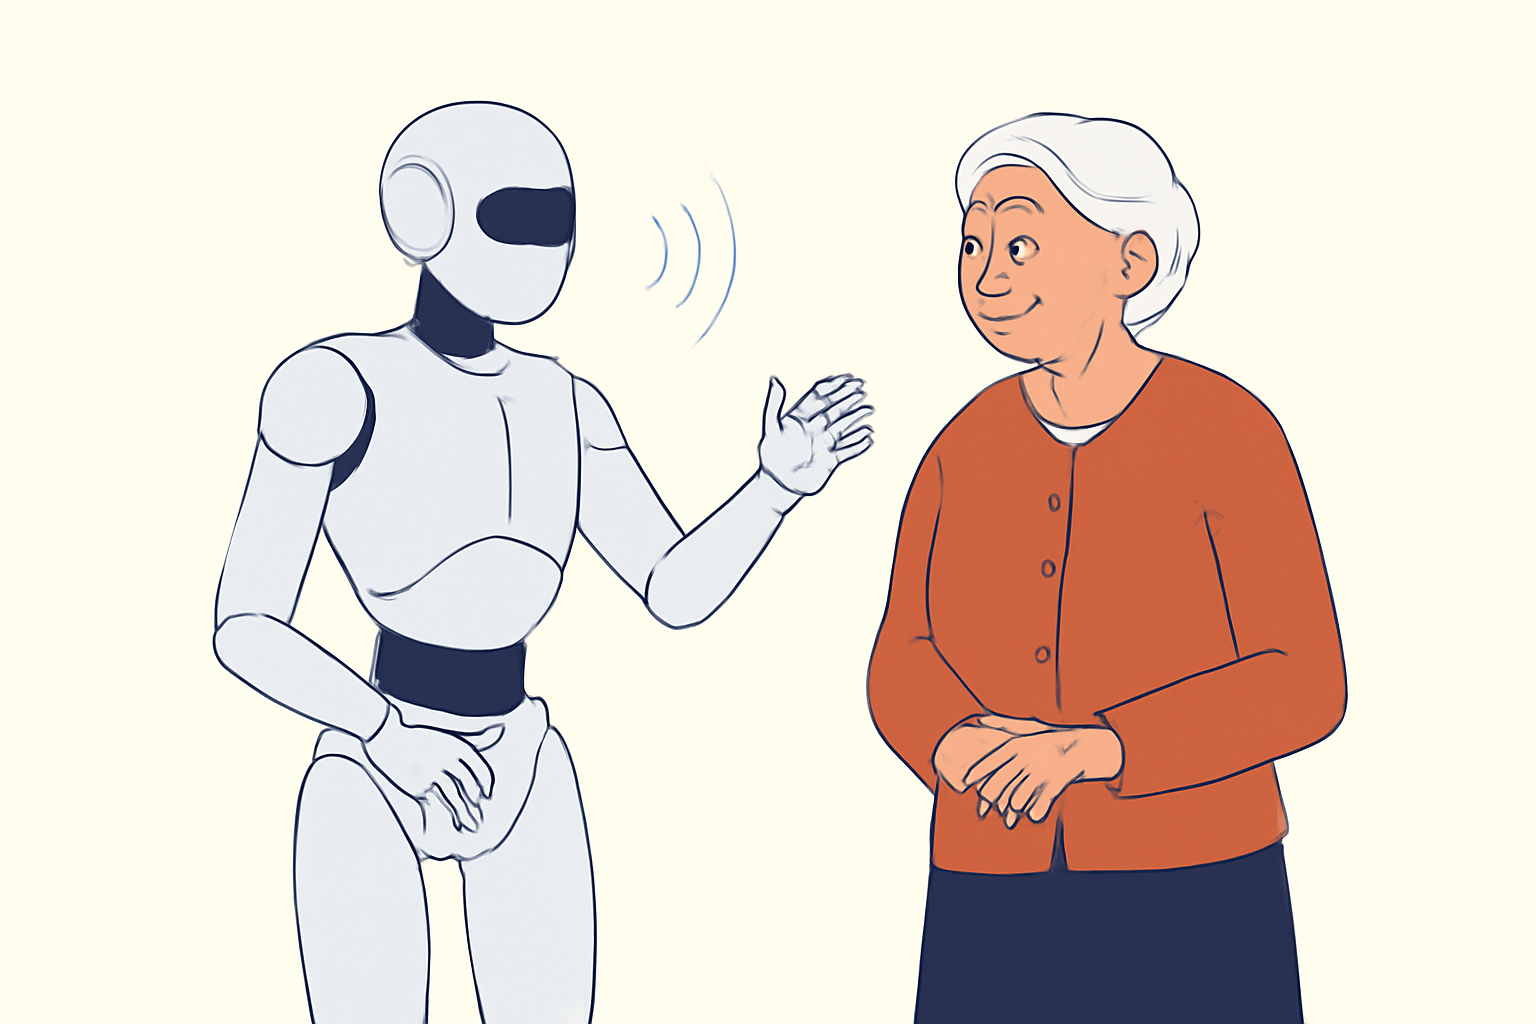
\includegraphics[width=0.95\linewidth,height=0.58\textheight,keepaspectratio]{images/tema_6/s02_por-que-conectamos-con-robots_img01.png}
    \end{column}
  \end{columns}
\end{frame}

\begin{frame}{Principios fundamentales}
  \small
  \begin{columns}[T,onlytextwidth]
    \begin{column}{0.58\textwidth}
      \begin{itemize}
        \item Percepción → cómo los robots usan sensores para reconocer la situación actual (contexto, voz, etc.)
        \item Empatía y emoción artificial → simulación de emociones para facilitar la interacción
        \item Comunicación no verbal → gestos, posturas y expresiones faciales
      \end{itemize}
    \end{column}
    \begin{column}{0.42\textwidth}
    \centering
    
\includegraphics[width=0.95\linewidth,height=0.58\textheight,keepaspectratio]{images/tema_6/s03_principios-fundamentales_img01.png}
    \end{column}
  \end{columns}
\end{frame}

\begin{frame}{Diseño centrado en el/la usuario/a}
  \small
  \begin{columns}[T,onlytextwidth]
    \begin{column}{0.58\textwidth}
      \begin{itemize}
        \item Los robots sociales deben ser diseñados pensando en cómo las personas interactúan con ellos, considerando factores como la accesibilidad, la empatía y la capacidad de adaptación
        \item Importancia de personalizar la interacción según las características y el contexto del usuario
      \end{itemize}
    \end{column}
    \begin{column}{0.42\textwidth}
    \centering
    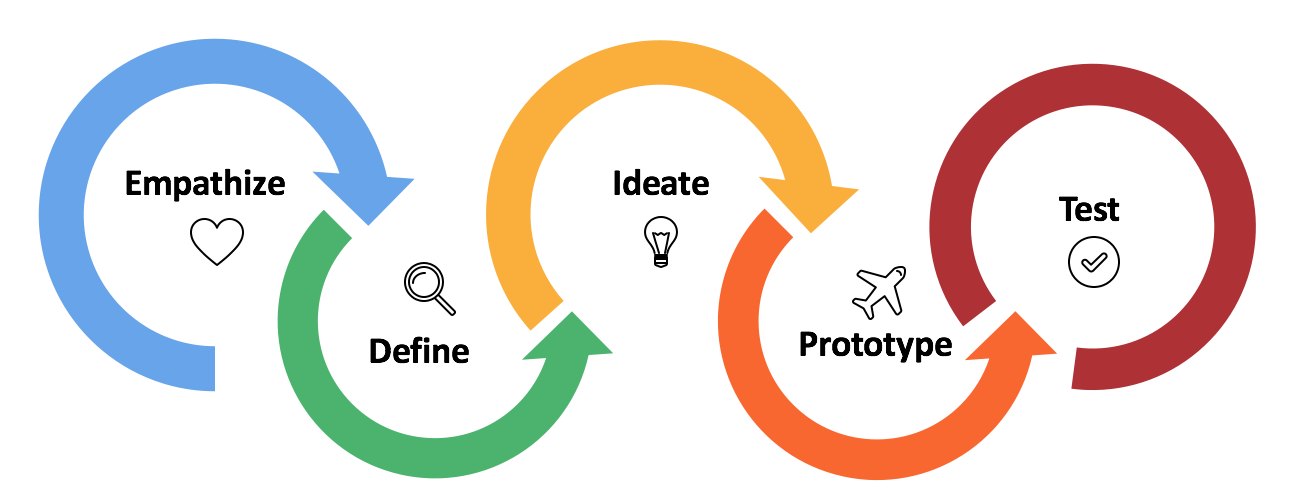
\includegraphics[width=0.95\linewidth,height=0.58\textheight,keepaspectratio]{images/tema_6/s04_diseno-centrado-en-el-la-usuario-a_img01.png}
    \end{column}
  \end{columns}
\end{frame}

\begin{frame}{Interacción multimodal}
  \small
  \begin{columns}[T,onlytextwidth]
    \begin{column}{0.58\textwidth}
      \begin{itemize}
        \item Diferentes canales → visual, auditivo, táctil
        \item Interacción más natural y fluida, como cuando un robot responde a un saludo con gesto y voz
      \end{itemize}
    \end{column}
    \begin{column}{0.42\textwidth}
    \centering
    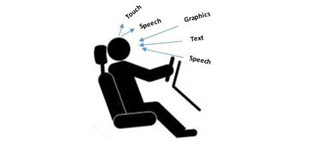
\includegraphics[width=0.95\linewidth,height=0.58\textheight,keepaspectratio]{images/tema_6/s05_interaccion-multimodal_img01.png}
    \end{column}
  \end{columns}
\end{frame}

\begin{frame}{Empatía artificial}
  \small
  \begin{columns}[T,onlytextwidth]
    \begin{column}{0.58\textwidth}
      \begin{itemize}
        \item $\rightarrow$ evocar y responder a emociones humanas,
        \item $\rightarrow$ identificar emociones humanas y generar respuestas empáticas
      \end{itemize}
      \begin{itemize}
        \item Los robots simulan emociones para facilitar la interacción
        \item Deben ‘sentir’ y responder a las emociones humanas para tratar de crear vínculos genuinos
        \item Diseño emocional:
      \end{itemize}
    \end{column}
    \begin{column}{0.42\textwidth}
    \centering
    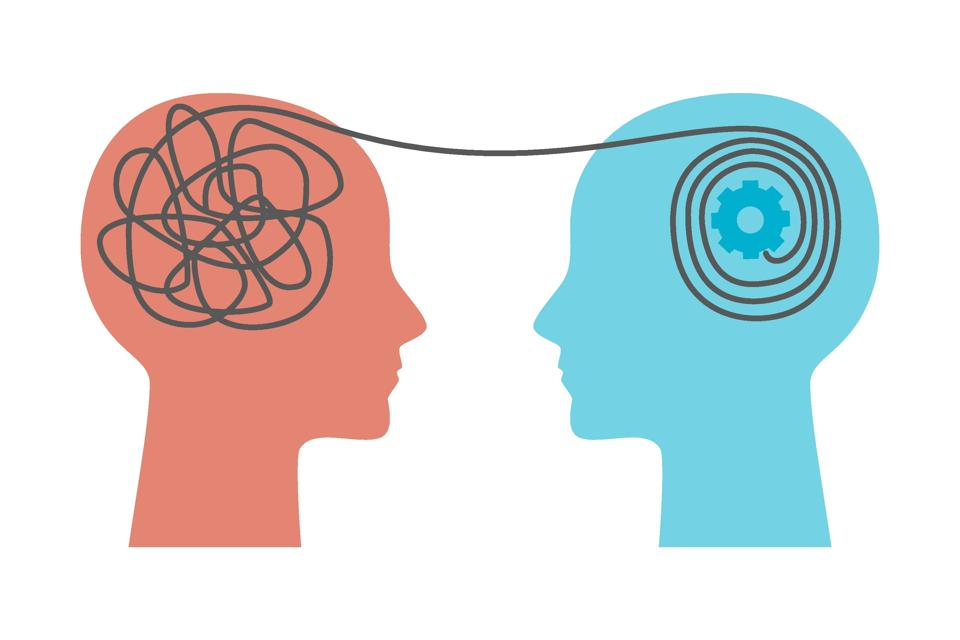
\includegraphics[width=0.95\linewidth,height=0.58\textheight,keepaspectratio]{images/tema_6/s06_empatia-artificial_img01.png}
    \end{column}
  \end{columns}
\end{frame}

\begin{frame}{Adaptación al contexto social}
  \small
  \begin{columns}[T,onlytextwidth]
    \begin{column}{0.58\textwidth}
      \begin{itemize}
        \item Los robots deben reconocer y adaptarse a los contextos sociales en los que interactúan
        \item Lo que implica ajustar sus respuestas tanto al entorno (hogar, hospital, escuela) como a las personas involucradas
      \end{itemize}
    \end{column}
    \begin{column}{0.42\textwidth}
    \centering
    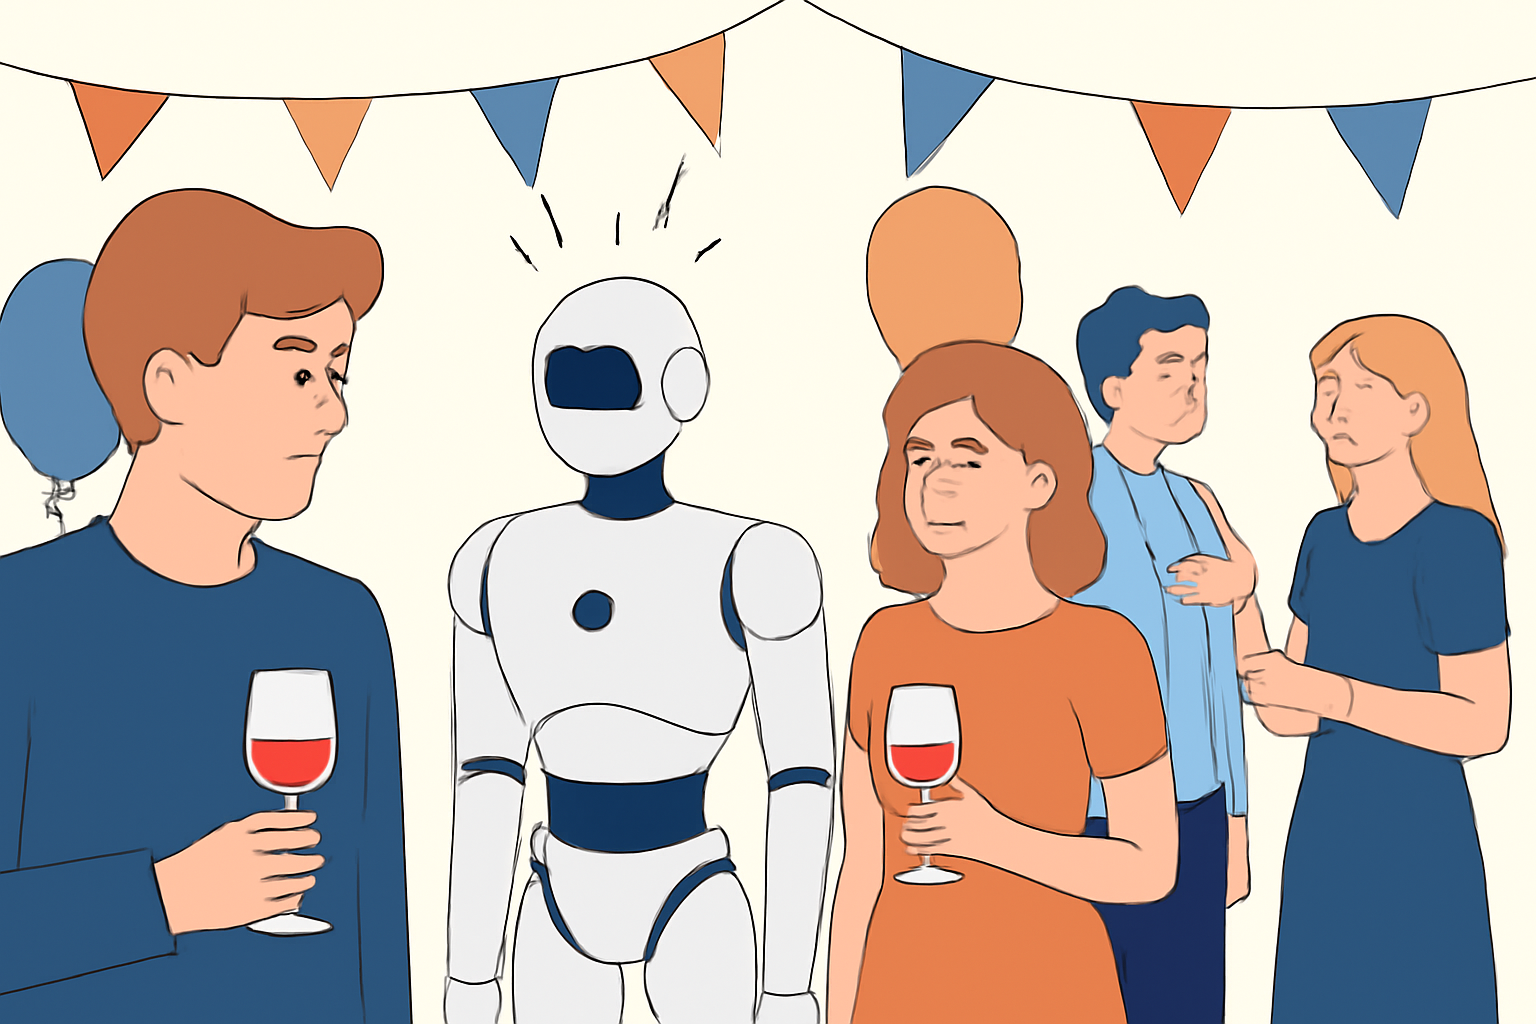
\includegraphics[width=0.95\linewidth,height=0.58\textheight,keepaspectratio]{images/tema_6/s07_adaptacion-al-contexto-social_img01.png}
    \end{column}
  \end{columns}
\end{frame}

\begin{frame}{Aceptación social}
  \small
  \begin{columns}[T,onlytextwidth]
    \begin{column}{0.58\textwidth}
      \begin{itemize}
        \item La aceptación social es crucial para que los robots sean utilizados
        \item Factores como la confianza, la apariencia y el comportamiento del robot influyen en la aceptación por parte de las personas
      \end{itemize}
    \end{column}
    \begin{column}{0.42\textwidth}
    \centering
    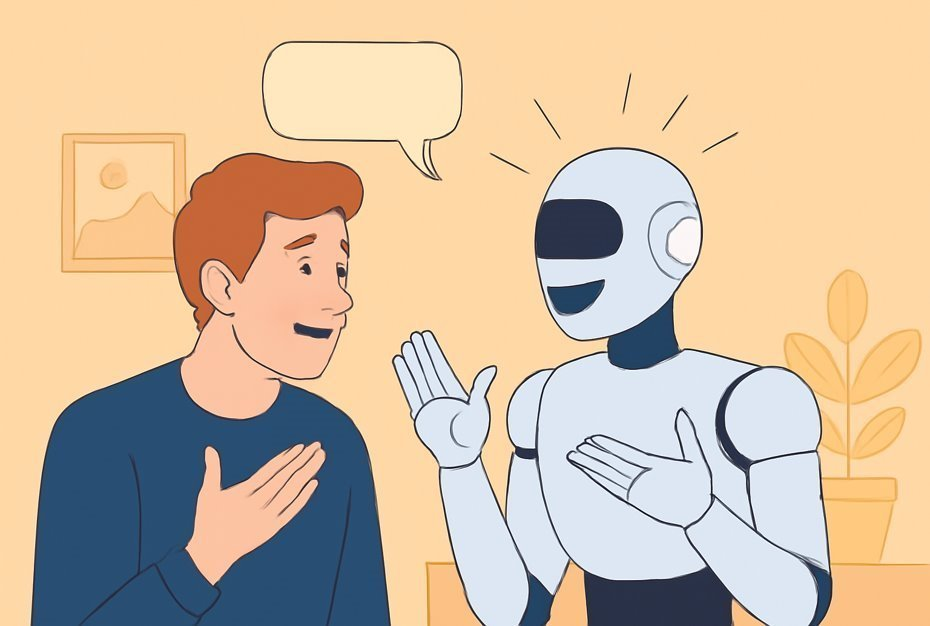
\includegraphics[width=0.95\linewidth,height=0.58\textheight,keepaspectratio]{images/tema_6/s08_aceptacion-social_img01.jpeg}
    \end{column}
  \end{columns}
\end{frame}

\begin{frame}{Evaluación de la respuesta emocional}
  \small
  \begin{columns}[T,onlytextwidth]
    \begin{column}{0.58\textwidth}
      \begin{itemize}
        \item Análisis facial, tono de voz y comportamiento no verbal de lxs usuarixs
        \item Ejemplo → EmoReact
      \end{itemize}
    \end{column}
    \begin{column}{0.42\textwidth}
    \centering
    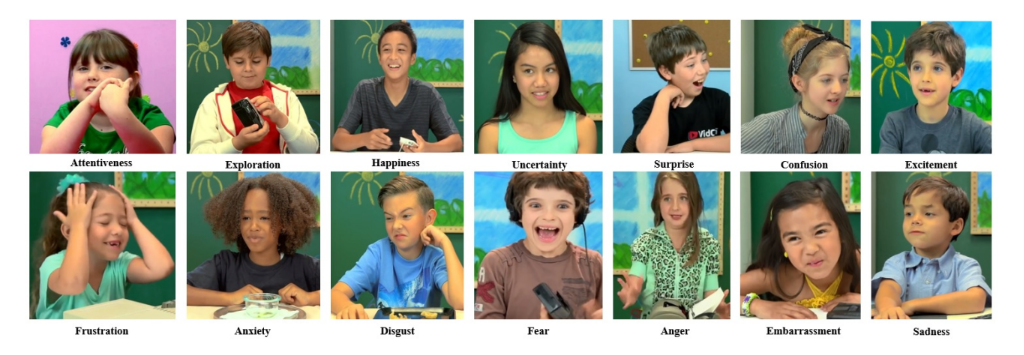
\includegraphics[width=0.95\linewidth,height=0.58\textheight,keepaspectratio]{images/tema_6/s09_evaluacion-de-la-respuesta-emocional_img01.png}
    \end{column}
  \end{columns}
\end{frame}

\begin{frame}{Ética}
  \small
  \begin{columns}[T,onlytextwidth]
    \begin{column}{0.58\textwidth}
      \begin{itemize}
        \item Los robots sociales pueden generar dependencia emocional en los usuarios (p.~ej., una persona anciana en soledad)
        \item ¿Deberían los robots tener derechos o protección contra el abuso humano?
      \end{itemize}
    \end{column}
    \begin{column}{0.42\textwidth}
    \centering
    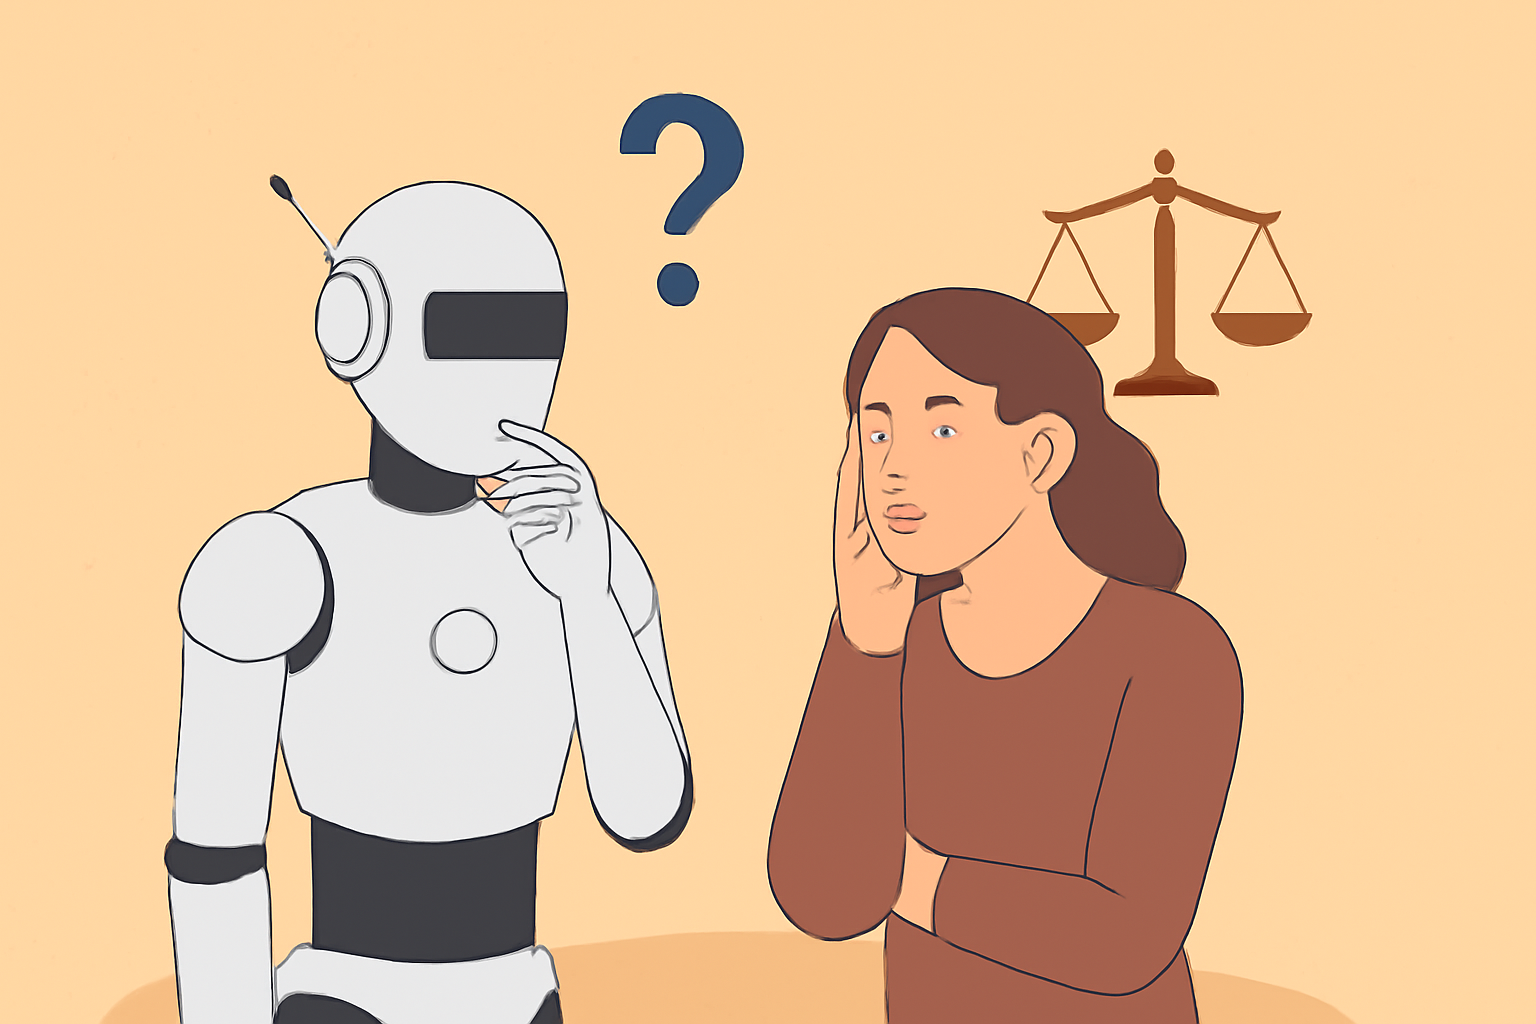
\includegraphics[width=0.95\linewidth,height=0.58\textheight,keepaspectratio]{images/tema_6/s10_etica_img01.png}
    \end{column}
  \end{columns}
\end{frame}

\begin{frame}{Desafíos}
  \small
  \begin{columns}[T,onlytextwidth]
    \begin{column}{0.58\textwidth}
      \begin{itemize}
        \item Percepción mutua
        \item Confianza
        \item Comunicación efectiva
        \item Expectativas vs. Realidad → limitaciones actuales en IA y robótica social
        \item Aspectos éticos y psicológicos → privacidad, confiabilidad, impacto psicológico
        \item Uncanny valley
      \end{itemize}
    \end{column}
    \begin{column}{0.42\textwidth}
    \centering
    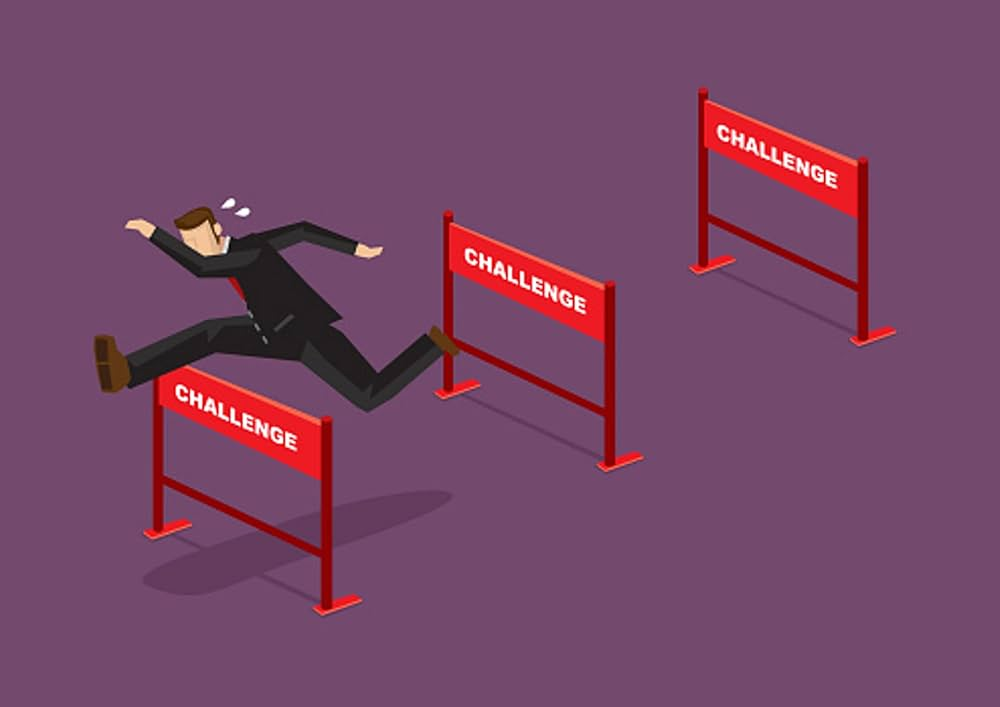
\includegraphics[width=0.95\linewidth,height=0.58\textheight,keepaspectratio]{images/tema_6/s11_desafios_img01.png}
    \end{column}
  \end{columns}
\end{frame}

\begin{frame}{Futuro}
  \small
  \begin{columns}[T,onlytextwidth]
    \begin{column}{0.58\textwidth}
      \begin{itemize}
        \item Mejoras en las capacidades de percepción y comprensión
        \item Avances en las regulaciones
        \item Impacto de la robótica social en el día a día
      \end{itemize}
    \end{column}
    \begin{column}{0.42\textwidth}
    \centering
    
\includegraphics[width=0.95\linewidth,height=0.58\textheight,keepaspectratio]{images/tema_6/s12_futuro_img01.png}
    \end{column}
  \end{columns}
\end{frame}

\section{Ejemplos (hri\_examples)}

\begin{frame}{Interacción humanx-robot}
  \small
  \begin{itemize}
    \item Máster Universitario en Ingeniería para la Discapacidad y la Rehabilitación
  \end{itemize}
\end{frame}

\end{document}
